\chapter{Материалы и методы исследования}
\label{sec:Chapter2} \index{Chapter2}

В данной главе приводится описание экспериментальной базы исследования, включая характеристики используемых наборов данных, формальную постановку задачи трансфера изображений, метрики количественной оценки качества синтезируемых изображений, а также базовые компоненты генеративно-состязательных сетей и функции потерь, применяемые в работе.
Представленные материалы и методы образуют фундамент для последующего анализа архитектурных решений, рассматриваемых в главе~\ref{sec:Chapter4}.

\section{Формальная постановка задачи}
\label{sec:problem_formulation}

Пусть имеется набор пар $\{(x_i, y_i)\}_{i=1}^N$, где $x_i \in \mathcal{X} \subset \mathbb{R}^{H \times W \times 1}$ -- входное радиолокационное изображение (одноканальное, нормированное), а $y_i \in \mathcal{Y} \subset \mathbb{R}^{H \times W \times 3}$ -- соответствующее ему эталонное оптическое RGB-изображение.
Требуется построить параметризованное отображение $G_\theta: \mathcal{X} \to \mathcal{Y}$, которое минимизирует некоторый функционал качества $\mathcal{L}(G_\theta(x), y)$, отражающий близость синтезированного изображения к реальному.
В контексте генеративно-состязательного обучения отображение $G_\theta$ (генератор) обучается совместно с дискриминатором $D_\phi$, решающим задачу бинарной классификации «реальное/сгенерированное».

\section{Метрики и функции потерь}
\label{sec:metrics_losses}

Для количественной оценки качества перевода радиолокационных изображений в оптические на основе генеративно-состязательных сетей применяются две группы инструментов: метрики оценки, вычисляемые на этапе тестирования и не влияющие на обучение, и функции потерь, определяющие целевую функцию оптимизации генератора $G$ и дискриминатора $D$.
Обе группы, в свою очередь, делятся на численные, то есть использующие прямые математические операции над пикселями или спектрами, и основанные на предобученных моделях, извлекающих высокоуровневые признаки.

\subsection{Метрики оценки качества}
\label{subsec:metrics}

Метрики служат для объективного сопоставления синтезированного изображения $\hat{y} = G(x)$ с эталонным оптическим снимком $y$.
Комплекс метрик охватывает попиксельные, структурные, частотные, перцептивные и семантические аспекты сходства.

\subsubsection{Численные метрики}

\paragraph{Среднеквадратичная ошибка (RMSE)}
Измеряет абсолютное отклонение яркостей пикселей:
\begin{equation}
\operatorname{RMSE}(y, \hat{y}) = \sqrt{\frac{1}{H W C} \sum_{i,j,k} (y_{ijk} - \hat{y}_{ijk})^2}.
\label{eq:rmse}
\end{equation}
Чем меньше значение RMSE, тем выше попиксельная точность восстановления.
Метрика чувствительна к выбросам, поэтому может переоценивать значимость крупных, но визуально малозаметных отклонений.

\paragraph{Пиковое отношение сигнал/шум (PSNR)}
Выражается в децибелах и обратно пропорционально логарифму среднеквадратичной ошибки:
\begin{equation}
\operatorname{PSNR}(y, \hat{y}) = 10 \log_{10}\left( \frac{\mathrm{MAX}^2}{\operatorname{MSE}} \right),
\label{eq:psnr}
\end{equation}
где $\mathrm{MAX} = 255$ для 8-битных изображений.
Более высокие значения PSNR соответствуют меньшим искажениям.
PSNR хорошо согласуется с попиксельной точностью, однако слабо коррелирует с визуальным восприятием текстур и мелких деталей.

\paragraph{Индекс структурного сходства (SSIM)}
SSIM \cite{wang2004image} моделирует особенности человеческого зрения, учитывая локальные изменения яркости, контраста и структуры:
\begin{equation}
\operatorname{SSIM}(y, \hat{y}) = \frac{(2\mu_y \mu_{\hat{y}} + C_1)(2\sigma_{y\hat{y}} + C_2)}{(\mu_y^2 + \mu_{\hat{y}}^2 + C_1)(\sigma_y^2 + \sigma_{\hat{y}}^2 + C_2)},
\label{eq:ssim}
\end{equation}
где $\mu$ -- среднее, $\sigma^2$ -- дисперсия, $\sigma_{y\hat{y}}$ -- ковариация; $C_1, C_2$ -- стабилизирующие константы.
Значения SSIM лежат в диапазоне $[-1, 1]$; близость к $1$ свидетельствует о высоком структурном сходстве.
Значение $-1$ означает, что сравниваемые изображения структурно полностью противоположны друг другу.
В контексте формулы SSIM это означает, что значения яркости пикселей двух картинок строго инвертированы относительно их среднего уровня.
SSIM лучше коррелирует с субъективной оценкой качества, чем PSNR.

\paragraph{Частотная ошибка (Frequency Domain Error, FDE)}
Попиксельные и структурные метрики часто не улавливают потерю высокочастотных текстур.
Для явного контроля спектральных характеристик вводится метрика в частотной области на основе двумерного быстрого преобразования Фурье (2D FFT) \cite{cai2021frequency}:
\begin{equation}
\operatorname{FDE}(y, \hat{y}) = \frac{1}{HW} \sum_{u=1}^{H} \sum_{v=1}^{W} \left| \log\left(|\mathcal{F}(y)_{uv}| + 1\right) - \log\left(|\mathcal{F}(\hat{y})_{uv}| + 1\right) \right|,
\label{eq:fde}
\end{equation}
где $\mathcal{F}(\cdot)$ -- двумерное преобразование Фурье, $|\cdot|$ -- модуль комплексной амплитуды. Логарифмическое масштабирование компенсирует большой динамический диапазон спектральных коэффициентов. Меньшее значение FDE указывает на более точное воспроизведение частотной структуры изображения. При необходимости спектр может быть разделён на низко- и высокочастотную области для раздельного анализа сохранности общей формы и мелких деталей.

\subsubsection{Метрики на основе предобученных моделей}

\paragraph{Перцептивное сходство (LPIPS)}
LPIPS \cite{zhang2018unreasonable} оценивает визуальное сходство, сравнивая карты признаков предобученной свёрточной сети (чаще всего AlexNet).
Для набора слоёв $l$ вычисляется взвешенная $\ell_2$-норма разности нормализованных активаций:
\begin{equation}
\operatorname{LPIPS}(y, \hat{y}) = \sum_l \frac{1}{H_l W_l} \sum_{h,w} \bigl\| w_l \odot (\phi_{hw}^l(y) - \phi_{hw}^l(\hat{y})) \bigr\|_2^2.
\label{eq:lpips}
\end{equation}
Меньшие значения LPIPS соответствуют большему визуальному сходству с точки зрения человека.
Метрика устойчива к небольшим пространственным сдвигам и изменениям текстуры, поэтому лучше отражает перцептивное качество, чем попиксельные аналоги.

\paragraph{Расстояние Фреше для признаков Inception (FID)}
FID \cite{heusel2017gans} измеряет различие между распределениями признаков реальных и сгенерированных изображений в пространстве внутренних слоев сети Inception-v3, в частности, предпоследнего слоя.
Предполагая многомерное нормальное распределение признаков, расстояние вычисляется как:
\begin{equation}
\operatorname{FID} = \|\mu_r - \mu_g\|_2^2 + \operatorname{Tr}\bigl(\Sigma_r + \Sigma_g - 2(\Sigma_r \Sigma_g)^{1/2}\bigr).
\label{eq:fid}
\end{equation}
Чем ниже FID, тем ближе статистические характеристики синтезированной выборки к реальным оптическим снимкам, что коррелирует с фотореалистичностью.
FID вычисляется на множестве изображений, поэтому оценивает качество генерации всей тестовой коллекции, а не отдельных пар.

\paragraph{Семантическая метрика SAMScore}
Традиционные метрики не учитывают сохранность семантических объектов (зданий, дорог, растительности, водоёмов).
SAMScore основана на предобученной модели сегментации Segment Anything Model (SAM) \cite{kirillov2023segment} и измеряет структурное сходство внутри автоматически выделяемых масок.
Вычисление состоит из двух шагов:
\begin{enumerate}
    \item Для эталонного оптического изображения $y$ SAM генерирует набор масок $\{M_k\}_{k=1}^{K}$, соответствующих семантически значимым регионам.
    \item Для каждой маски $M_k$ вычисляется показатель структурного сходства SSIM~\ref{eq:ssim} между $y$ и $\hat{y}$ в пределах этой маски.
\end{enumerate}
Итоговая метрика -- средневзвешенное значение по площадям масок:
\begin{equation}
\operatorname{SAMScore}(y, \hat{y}) = \frac{1}{\sum_{k=1}^{K} |M_k|} \sum_{k=1}^{K} |M_k| \cdot \operatorname{SSIM}\bigl(y \odot M_k,\; \hat{y} \odot M_k\bigr),
\label{eq:samscore}
\end{equation}
где $|M_k|$ -- площадь маски, $\odot$ -- поэлементное умножение. SAMScore $\in [0,1]$, и более высокие значения свидетельствуют о лучшем сохранении семантической структуры сцены. Метрика особенно информативна, когда критично правильное воспроизведение объектов определённых классов.

\subsection{Функции потерь}
\label{subsec:losses}
Обучение генератора $G$ осуществляется путём минимизации составной функции потерь, объединяющей несколько компонент, каждая из которых отвечает за определённый аспект качества перевода.
Все используемые потери являются дифференцируемыми по выходному изображению $\hat{y} = G(x)$, что является необходимым условием для обучения нейронной сети методом обратного распространения ошибки.

\subsubsection{Численные потери}

\paragraph{Пиксельные потери}
$\ell_1$-потеря (средняя абсолютная ошибка) и $\ell_2$-потеря (среднеквадратичная ошибка) накладывают прямое ограничение на попиксельное соответствие:
\begin{equation}
\mathcal{L}_{\ell_1} = \frac{1}{HWC} \sum |y - G(x)|, \quad \mathcal{L}_{\ell_2} = \frac{1}{HWC} \sum (y - G(x))^2.
\label{eq:l1_l2}
\end{equation}
$\ell_1$ менее чувствительна к выбросам и способствует сохранению резких границ, тогда как $\ell_2$ склонна излишне сглаживать изображение.
В задаче трансляции РЛИ в оптический диапазон обычно предпочтение отдаётся $\ell_1$-норме.

\paragraph{Состязательная потеря (Adversarial Loss)}
Определяет взаимодействие генератора и дискриминатора в минимаксной игре.
В работе может применяться один из вариантов:
\begin{itemize}
    \item Классическая кросс-энтропия:
    \begin{equation}
        \mathcal{L}_{\text{adv},G} = -\mathbb{E}[\log D(G(x))].
        \label{eq:adv_loss}
    \end{equation}
    \item Потеря наименьших квадратов (LSGAN) \cite{mao2017least}:
    \begin{equation}
        \mathcal{L}_{\text{adv},G} = \frac{1}{2}\mathbb{E}[(D(G(x))-1)^2].
        \label{eq:lsgan_loss}
    \end{equation}
    \item Hinge loss:
    \begin{equation}
        \mathcal{L}_{\text{adv},G} = -\mathbb{E}[D(G(x))].
        \label{eq:hinge_loss}
    \end{equation}
\end{itemize}

Состязательная потеря побуждает генератор создавать изображения, неотличимые дискриминатором от реальных оптических снимков, повышая их фотореалистичность.

\paragraph{Потеря сопоставления признаков (Feature Matching Loss)}
Для стабилизации состязательного обучения и обогащения градиентного сигнала в работе используется потеря сопоставления признаков, вычисляемая по промежуточным картам активаций дискриминатора:
\begin{equation}
\mathcal{L}_{\text{FM}} = \sum_{i=1}^{T} \frac{1}{N_i} \bigl\| D^{(i)}(x, y) - D^{(i)}(x, G(x)) \bigr\|_1,
\label{eq:fm_loss}
\end{equation}
где $D^{(i)}(\cdot)$ -- активации $i$-го промежуточного слоя дискриминатора, $N_i$ -- число элементов в этом слое, $T$ -- общее число учитываемых слоёв.
В отличие от чисто состязательного сигнала, эта потеря требует от генератора воспроизводить статистики признаков на всех уровнях иерархии дискриминатора, что сглаживает оптимизационный ландшафт и снижает риск моделирующих коллапсов, характерных для GAN.

\paragraph{Частотная потеря (Frequency Loss)}
Для явного контроля спектральных характеристик вводится потеря, минимизирующая разность логарифмированных амплитудных Фурье-спектров, аналогичная метрике FDE:
\begin{equation}
\mathcal{L}_{\text{freq}} = \frac{1}{HW} \sum_{u,v} \bigl| \log(|\mathcal{F}(y)_{uv}| + 1) - \log(|\mathcal{F}(G(x))_{uv}| + 1) \bigr|.
\label{eq:freq_loss}
\end{equation}

Данная потеря стимулирует генератор восстанавливать высокочастотные текстуры, предотвращая чрезмерную сглаженность, характерную для моделей, оптимизируемых только по пиксельным критериям.

\subsubsection{Потери на основе предобученных моделей}

\paragraph{Перцептивная потеря на основе VGG (Perceptual Loss)}
Классическая перцептивная потеря \cite{johnson2016perceptual} использует предобученную сеть VGG-19 для сравнения карт признаков реального и синтезированного изображений:
\begin{equation}
\mathcal{L}_{\text{perc}} = \sum_{l} \lambda_l \bigl\| \phi_l(y) - \phi_l(G(x)) \bigr\|_1,
\label{eq:perc_loss}
\end{equation}
где $\phi_l$ -- активации $l$-го свёрточного слоя, $\lambda_l$ -- весовые коэффициенты.
Перцептивная потеря смягчает требование точного попиксельного совпадения, поощряя генерацию визуально убедительных текстур и семантически осмысленных структур.

\paragraph{Перцептивная потеря на основе DINOv2}
Современные самоконтролируемые модели зрения, такие как DINOv2 \cite{oquab2023dinov2}, формируют семантически более насыщенные и устойчивые к несущественным вариациям представления.
DINOv2-потеря вычисляется как взвешенная сумма $\ell_1$-расстояний между признаками, извлечёнными из нескольких блоков трансформера (например, ViT-B/14):
\begin{equation}
\mathcal{L}_{\text{DINOv2}} = \sum_{b \in \mathcal{B}} \lambda_b \bigl\| \phi_b(y) - \phi_b(G(x)) \bigr\|_1,
\label{eq:dinov2_loss}
\end{equation}
где $\phi_b(\cdot)$ -- выход $b$-го блока, $\mathcal{B}$ -- множество выбранных блоков, $\lambda_b$ -- веса. Признаки DINOv2 лучше отражают глобальную структуру сцены и семантическую принадлежность объектов, благодаря чему данная потеря обеспечивает высокую корреляцию с субъективным качеством и может превосходить VGG-потерю в задачах трансляции изображений.

\paragraph{Семантическая потеря на основе SAM (SAM Loss)}
Для акцентирования внимания генератора на значимых объектах вводится потеря, использующая маски, автоматически сгенерированные моделью SAM.
В отличие от метрики SAMScore, где вычисляется SSIM, в качестве обучающего сигнала применяется взвешенная $\ell_1$-норма внутри масок:
\begin{equation}
\mathcal{L}_{\text{SAM}} = \frac{1}{\sum |M_k|} \sum_k \bigl\| (y - G(x)) \odot M_k \bigr\|_1.
\label{eq:sam_loss}
\end{equation}
Такой подход направляет оптимизацию на точное восстановление семантически значимых регионов, таких как здания, дороги и водоёмы, улучшая интерпретируемость результата.

\subsubsection{Полная целевая функция генератора}
Общая функция потерь генератора представляет собой линейную комбинацию описанных компонент:
\begin{equation}
\mathcal{L}_G = \lambda_{\ell_1} \mathcal{L}_{\ell_1} + \lambda_{\text{adv}} \mathcal{L}_{\text{adv}} + \lambda_{\text{perc}} \mathcal{L}_{\text{perc}} + \lambda_{\text{DINOv2}} \mathcal{L}_{\text{DINOv2}} + \lambda_{\text{freq}} \mathcal{L}_{\text{freq}} + \lambda_{\text{SAM}} \mathcal{L}_{\text{SAM}}.
\label{eq:loss_function}
\end{equation}
Веса $\lambda$ подбираются экспериментально для достижения баланса между попиксельной точностью, перцептивным качеством, спектральной достоверностью и семантической согласованностью.
Применение многокомпонентной функции потерь является стандартной практикой в задачах перевода изображений и позволяет превзойти модели, обученные только по $\ell_1$ или $\ell_2$ норме.

\subsection{Дифференцируемость компонент}
\label{subsec:differentiability}

Все функции потерь, входящие в состав $\mathcal{L}_G$~\ref{eq:loss_function}, являются дифференцируемыми (или субдифференцируемыми) по выходу генератора $\hat{y}$ в рамках используемого программного стека с автоматическим дифференцированием:
\begin{itemize}
    \item $\ell_1$ и $\ell_2$ -- гладкие (или допускающие субградиент) попиксельные функции.
    \item Состязательная потеря дифференцируема при фиксированном дискриминаторе $D$, поскольку $D$ -- нейросеть с непрерывно-дифференцируемыми активациями.
    \item Перцептивные потери VGG и DINOv2 опираются на прямое распространение через предобученные сети, веса которых заморожены; все операции (свёртки, нормализации, внимание в трансформере) дифференцируемы.
    \item Частотная потеря $\mathcal{L}_{\text{freq}}$ реализуется через композицию БПФ (линейный оператор), взятия модуля, логарифма и $\ell_1$; все эти операции поддерживают вычисление градиента в PyTorch, поэтому потеря полностью дифференцируема.
    \item SAM-потеря использует предварительно извлечённые маски $M_k$, которые фиксированы и не зависят от генератора; поэлементное умножение на маску и $\ell_1$ дифференцируемы.
\end{itemize}

Метрики оценки (RMSE, PSNR, SSIM, FDE, LPIPS, SAMScore) также дифференцируемы, но в рамках данной работы они не используются при обучении (за исключением случаев, когда LPIPS или его аналоги явно включаются в функцию потерь).
FID является недифференцируемой метрикой, так как опирается на статистики по батчу и требует вычисления квадратного корня из матрицы для всей выборки, что не позволяет вычислить градиент для отдельного изображения.
Поэтому FID применим исключительно для итоговой оценки качества генерации.

\subsection{Сводная таблица}
Для удобства сопоставления все рассмотренные метрики и функции потерь сведены в таблицу~\ref{tab:metrics_losses_summary}.

\begin{table}[H]
\centering
\caption{Сводная таблица метрик и функций потерь}
\label{tab:metrics_losses_summary}
\renewcommand{\arraystretch}{1.2}
\begin{tabular}{l p{2.0cm} p{1.5cm} p{7.5cm}}
\toprule
\textbf{Метрика / Потеря} & \textbf{Тип} & \textbf{Дифф.} & \textbf{Назначение и особенности} \\
\midrule
\multicolumn{4}{l}{\textit{Метрики оценки (не применяются при обучении)}} \\
\midrule
RMSE, PSNR & Численная & Да & Абсолютная попиксельная точность; PSNR в дБ. Не всегда коррелируют с восприятием. \\
SSIM & Численная & Да & Структурное сходство; учитывает локальные изменения яркости и контраста. Хорошо согласуется с экспертной оценкой. \\
FDE & Численная & Да & Спектральное сходство; логарифмическая разность амплитудных Фурье-спектров. Оценивает сохранность текстур и мелких деталей. \\
LPIPS & Модельная (AlexNet/VGG) & Да & Перцептивное сходство; сравнивает признаки предобученной CNN. Может также использоваться как функция потерь. \\
FID & Модельная (Inception-v3) & Нет & Статистическое расстояние между распределениями признаков; оценивает реалистичность всей выборки. Недифференцируем. \\
SAMScore & Модельная (SAM) & Да & Семантическое структурное сходство; средневзвешенный SSIM внутри масок объектов. \\
\midrule
\multicolumn{4}{l}{\textit{Функции потерь (минимизируются при обучении генератора)}} \\
\midrule
\(\mathcal{L}_{\ell_1}\) / \(\mathcal{L}_{\ell_2}\) & Численная & Да & Попексельное восстановление; \(\ell_1\) предпочтительнее для сохранения границ. \\
\(\mathcal{L}_{\text{adv}}\) & Численная (через \(D\)) & Да & Состязательная игра; повышает фотореалистичность синтезированных изображений. \\
\(\mathcal{L}_{\text{perc}}\) (VGG) & Модельная (VGG) & Да & Перцептивная близость; использует признаки свёрточной сети. Смягчает попиксельные требования. \\
\(\mathcal{L}_{\text{DINOv2}}\) & Модельная (DINOv2) & Да & Перцептивная потеря на основе самоконтролируемого ViT. Улучшает глобальную структуру и семантику. \\
\(\mathcal{L}_{\text{freq}}\) & Численная & Да & Частотная согласованность; минимизирует разность Фурье-спектров. Предотвращает переглаживание. \\
\(\mathcal{L}_{\text{SAM}}\) & Модельная (SAM-маски) & Да & Взвешенная \(\ell_1\) внутри масок семантических объектов. Акцентирует значимые регионы. \\
\bottomrule
\end{tabular}
\end{table}

\section{Используемые наборы данных}
\label{sec:datasets}

Для обучения и валидации моделей трансфера SAR $\rightarrow$ Optical в работе задействованы два открытых набора данных, получивших широкое признание в сообществе исследователей дистанционного зондирования Земли: SEN1-2 \cite{schmitt2018sen1} и QXS-SAROPT \cite{huang2021qxs}.
Оба датасета предоставляют пары предварительно обработанных и геометрически совмещённых изображений радиолокационного и оптического диапазонов, что позволяет сосредоточиться на разработке и сравнительном анализе архитектур генеративных нейронных сетей.

\subsection{Датасет SEN1-2}
\label{subsec:sen1-2}

Датасет SEN1-2 \cite{schmitt2018sen1}, опубликованный в 2018 году, является одним из наиболее репрезентативных публичных ресурсов для задач кросс-модального обучения в дистанционном зондировании.
Он содержит 282\,384 строго зарегистрированные пары фрагментов размером $256 \times 256$ пикселей, полученных спутниками Sentinel-1 (радиолокационный канал) и Sentinel-2 (оптический канал).
Ключевой особенностью датасета является глобальный охват: фрагменты распределены по всем континентам и охватывают четыре метеорологических сезона, что обеспечивает высокую вариативность ландшафтов, типов земного покрова и условий освещения.

\paragraph{Физическая природа и формат радиолокационных данных.}
Радиолокационные фрагменты (папки \texttt{s1\_i}) представляют собой одноканальные 8-битные изображения в формате PNG.
Исходные значения коэффициента нормализованного обратного рассеяния $\sigma^0$ (sigma nought) предварительно конвертируются в децибельную шкалу:
\begin{equation}
    \sigma^0_{\text{dB}} = 10 \cdot \log_{10}(\sigma^0_{\text{linear}}),
\end{equation}
после чего выполняется линейное масштабирование в диапазон $[0, 255]$ для совместимости со стандартными форматами хранения изображений.
Используется вертикальная поляризация (VV), диапазон частот C-band ($\sim$5.405 ГГц), режим съёмки Interferometric Wide Swath (IW) с пространственным разрешением $\sim$10 м после мульти-выглядения (multilooking) \cite{schmitt2018sen1}.
Такая предобработка сохраняет динамический диапазон, характерный для радиолокационных данных, но требует обратной нормализации при обучении нейросетевых моделей.

\paragraph{Оптические данные и атмосферная коррекция.}
Оптические фрагменты (папки \texttt{s2\_i}) представляют собой трёхканальные композиты спектральных каналов Sentinel-2: B4 (Red, 665 нм), B3 (Green, 560 нм) и B2 (Blue, 490 нм) с пространственным разрешением 10 м.
Все изображения прошли атмосферную коррекцию уровня L2A (Bottom-Of-Atmosphere reflectance), что минимизирует влияние аэрозолей и молекулярного рассеяния и обеспечивает физическую согласованность спектральных характеристик \cite{schmitt2018sen1}.
Данные хранятся в формате 8-битных PNG-изображений с линейным масштабированием коэффициентов отражения.

\paragraph{Структура и лицензирование.}
Датасет организован иерархически: на верхнем уровне расположены четыре папки, соответствующие метеорологическим сезонам (\texttt{ROIs1158\_spring}, \texttt{ROIs1868\_summer}, \texttt{ROIs1970\_fall}, \texttt{ROIs2017\_winter}), внутри которых сгруппированы сцены по идентификаторам.
Распространение осуществляется под лицензией CC-BY 4.0.

\paragraph{Выбор подмножества для экспериментов.}
В рамках данного исследования с учётом вычислительных ограничений, используется подмножество весеннего сезона (\texttt{ROIs1158\_spring}).
Из полного набора сцен отобраны девять репрезентативных регионов: S5, S10, S25, S35, S45, S47, S52, S84 и S100.
Данный выбор обусловлен следующими факторами:
\begin{itemize}
    \item \textbf{Разнообразие классов земного покрова:} отобранные сцены включают плотную городскую застройку, пригородные зоны, сельскохозяйственные угодья, водные объекты и холмистый рельеф, что позволяет оценить обобщающую способность модели на разнородных данных;
    \item \textbf{Сопоставимость с базовыми работами:} использование того же подмножества обеспечивает корректное сравнение с результатами, представленными в работе \cite{wei2023cfrwd};
    \item \textbf{Баланс объёма и качества:} итоговое подмножество содержит $\sim$20\,000 пар изображений, что сопоставимо с объёмом датасета QXS-SAROPT \cite{huang2021qxs} и достаточно для устойчивого обучения без избыточных вычислительных затрат.
\end{itemize}

Разбиение на обучающую и тестовую выборки выполнено в соотношении $4:1$ с сохранением пропорционального представительства классов сцен.

\paragraph{Предобработка данных и аугментации.}
\label{par:preprocessing_augmentations}

Перед подачей в модель исходные 8-битные изображения нормализуются к диапазону $[-1, 1]$ посредством линейного преобразования:
\begin{equation}
    x_{\text{norm}} = 2 \cdot \frac{x - x_{\min}}{x_{\max} - x_{\min}} - 1,
    \label{eq:normalization}
\end{equation}
где $x_{\min}=0$, $x_{\max}=255$. Данная нормализация обеспечивает численную стабильность оптимизации и согласованность с областью определения активационной функции $\tanh$ на выходном слое генератора.

\subparagraph{Базовые аугментации.}
В процессе обучения применяется набор детерминированных геометрических преобразований, повышающих инвариантность модели к ориентации сцены:
\begin{itemize}
    \item случайные горизонтальные и вертикальные отражения;
    \item повороты на углы, кратные $90^\circ$ ($90^\circ$, $180^\circ$, $270^\circ$).
\end{itemize}
Указанные преобразования не искажают спектральные характеристики изображений и не требуют интерполяции пикселей (за исключением поворотов, где применяется ближайший сосед или билинейная интерполяция с последующим округлением до целых значений), что сохраняет целостность радиометрической информации.

\subparagraph{Опциональные стохастические аугментации.}
Для повышения робастности модели к вариациям съёмки и снижения риска переобучения дополнительно могут применяться следующие преобразования с вероятностью $p \in [0.3, 0.5]$:
\begin{itemize}
    \item \textbf{Мультипликативный шум.} Добавление мультипликативного шума с относительной амплитудой до $10\%$ ($x' = x \cdot (1 + \varepsilon)$, $\varepsilon \sim \mathcal{N}(0, 0.1^2)$), имитирующее флуктуации радиометрической калибровки и атмосферные помехи;
    \item \textbf{Малые аффинные искажения.} Повороты на угол $\delta \in [-5^\circ, 5^\circ]$ и масштабирование с коэффициентом $s \in [0.9, 1.1]$, моделирующие неточности геопривязки и вариации масштаба съёмки;
    \item \textbf{Случайное кадрирование.} Обрезка фрагмента изображения с уменьшением линейных размеров до $10\%$ с последующим ресайзом к исходному разрешению, что способствует обучению модели локальным признакам и снижает зависимость от глобального контекста.
    \item \textbf{Случайное перемещаение.} Транслирование изображения на относительное значение до 5\% по двум осям. В пересчете для датасета с изображениями $256 \times 256$ получаем случайное перемещение $\Delta x \in [-12.6; 12.6], \Delta y \in [-12.6; 12.6]$.
\end{itemize}

\subparagraph{Обработка граничных артефактов.}
Все аугментации, сопровождающиеся появлением областей, не покрытых исходным изображением (например, при поворотах или масштабировании), реализуются с использованием зеркального заполнения (reflection padding).
Данный выбор обусловлен физической природой радиолокационных данных: заполнение нулевыми (чёрными) пикселями вводит в обучающую выборку нефизичные паттерны (рис.~\ref{fig:qxs-saropt_sar_opt_affine_artifact_example}), не соответствующие реальному распределению обратного рассеяния, и может провоцировать артефакты генерации на границах сцены.
Зеркальное продолжение, напротив, сохраняет локальную статистику текстур и градиентов, минимизируя разрывы на границах и улучшая обобщающую способность модели.
Хотя зеркальное заполнение и восстанавливает недостающие части изображений, их природа по-прежнему остается нефизичной, что также препятствует корректному обучению модели.
Именно поэтому данные аугментации вынесены в опциональные.

\subparagraph{Стратегия применения.}
Для сохранения строгой пиксельной корреляции между модальностями трансформации применяются синхронно к паре изображений (РЛИ и оптическое).
В рамках каждой итерации обучения параметры стохастических аугментаций (угол поворота, коэффициент масштабирования, реализация мультипликативного шума) фиксируются на уровне псевдослучайных чисел и транслируются на оба канала без изменений.
Такой подход гарантирует, что геометрические и радиометрические искажения вносятся согласованно, не нарушая условную зависимость $p(y_{\text{opt}} \mid x_{\text{SAR}})$, заложенную при формировании датасета.

Дополнительно исследовались сценарии асимметричной аугментации, при которой геометрические или фотометрические искажения применялись исключительно к радиолокационному входу.
Это может повысить робастность модели к временному рассогласованию снимков.
Однако на практике подобная стратегия приводила к семантическому рассогласованию признакового пространства: модель начинала интерпретировать искусственные искажения SAR-изображения как физические изменения ландшафта, что провоцировало нестабильность состязательного обучения и требовало кратно более сложной настройки гиперпараметров и введения дополнительных ограничений на пространственную инвариантность.
В связи с этим был выбран консервативный подход строгой синхронизации

\subsection{Датасет QXS-SAROPT}
\label{subsec:qxs-saropt}

Датасет QXS-SAROPT \cite{huang2021qxs}, представленный в 2021 году, является специализированным набором данных для задач кросс-модального перевода в условиях высокой детализации.
Он включает 20\,000 строго зарегистрированных пар фрагментов размером $256 \times 256$ пикселей с пространственным разрешением 1 м/пиксель.
В отличие от глобально ориентированного SEN1-2, данный датасет сфокусирован на урбанизированных прибрежных территориях трёх мегаполисов: Циндао (Китай), Шанхай (Китай) и Сан-Диего (США).
Такая географическая специфика обеспечивает высокую концентрацию сложных антропогенных объектов (портовая инфраструктура, маломерные суда, транспортные развязки, плотная застройка), что делает датасет ценным бенчмарком для оценки способности моделей восстанавливать высокочастотные детали и мелкомасштабную семантику.

\paragraph{Физическая природа и формат радиолокационных данных.}
Радиолокационные фрагменты получены китайским спутником Gaofen-3, оснащённым C-диапазонным ($\sim$5.4 ГГц) SAR-сенсором.
В отличие от режима Interferometric Wide Swath (Sentinel-1), Gaofen-3 работает в режиме Spotlight, обеспечивающем повышенное пространственное разрешение за счёт управления диаграммой направленности антенны в течение времени экспозиции.
Используется однополяризационная конфигурация (преимущественно VV), данные представлены в виде одноканальных 8-битных изображений в формате PNG.
Исходные значения коэффициента обратного рассеяния $\sigma^0$ предварительно линеаризованы и масштабированы в диапазон $[0, 255]$ с сохранением динамического диапазона, характерного для городских сцен с высокой контрастностью (металлические конструкции, угловые отражатели, водные поверхности).

\paragraph{Оптические данные и процедура регистрации.}
Оптические фрагменты извлечены из сервиса Google Earth и представляют собой трёхканальные композиты в цветовой модели RGB.
Все пары прошли процедуру точной пространственной корреляции (сорегистрации) с субпиксельной точностью, которые встречаются в SEN1-2, что минимизирует геометрические рассогласования, критичные для обучения парных моделей.
Оптические изображения также масштабированы к 8-битному представлению и приведены к единому разрешению 1 м/пиксель.
Важно отметить, что, в отличие от уровней обработки L2A Sentinel-2, оптические данные из Google Earth могут содержать следы постобработки (резкость, баланс белого, компрессия), что вносит дополнительный доменный сдвиг и повышает требования к робастности моделей.

Важно отметить, что в отличие от SEN1-2, в QXS-SAROPT встречаются ранее описанные граничные артефакты, в частности от афинных преобразований (поворота и трансляции)

\begin{figure}[!ht]
    \centering
    \begin{subfigure}[t]{0.4\textwidth}
        \centering
        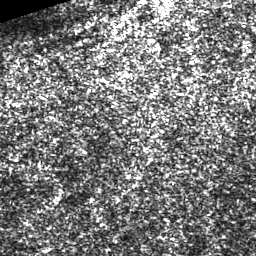
\includegraphics[width=\textwidth]{./images/qxs_sar2opt/296_sar.png}
        \caption{Радиолокационное изображение QXS-SAROPT c граничными артефактами}
        \label{subfig:qxs-saropt_sar_affine_artifact_example}
    \end{subfigure}
    \hspace{0.5cm}
    \begin{subfigure}[t]{0.4\textwidth}
        \centering
        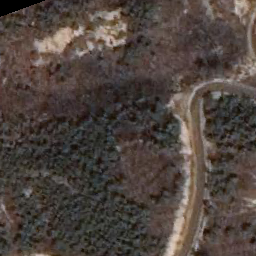
\includegraphics[width=\textwidth]{./images/qxs_sar2opt/296_opt.png}
        \caption{Оптическое RGB-изображение QXS-SAROPT с граничными артефактами}
        \label{subfig:qxs-saropt_opt_affine_artifact_example}
    \end{subfigure}
    \caption{Пример изображения из датасета QXS-SAROPT с граничными артефактами, возникающими при аффинных преобразованиях (левый верхний угол).}
    \label{fig:qxs-saropt_sar_opt_affine_artifact_example}
\end{figure}

\paragraph{Структура и лицензирование.}
Датасет организован в виде корневых папок \texttt{sar\_256\_oc\_0.2} и \texttt{opt\_256\_oc\_0.2}, внутри которых хранятся изображения.
Распространение осуществляется под лицензией, допускающей некоммерческое исследовательское использование.

\paragraph{Выбор подмножества и стратегия аугментации.}
В рамках данного исследования используется полный объём датасета с сохранением авторского разбиения 4:1.
Аугментации применяются синхронно к парам изображений и идентичны описанным в подразделе~\ref{par:preprocessing_augmentations} для SEN1-2: базовые геометрические преобразования (отражения, повороты на $90^\circ$) и опциональные стохастические аугментации.

\paragraph{Нормализация.}
Перед подачей в модель данные нормализуются к диапазону $[-1, 1]$ посредством линейного преобразования~\eqref{eq:normalization}.
Для оптических изображений дополнительно применяется проверка на артефакты компрессии JPEG (блоки 8×8), которые могут влиять на вычисление перцептивных метрик (LPIPS~\ref{eq:lpips}) и требуют аккуратной интерпретации результатов.

\subsection{Сводная характеристика датасетов}
\label{subsec:datasets_summary}
В данном исследовании используются два общедоступных датасета: SEN1-2 и QXS-SAROPT.
Выбор обусловлен их комплементарностью: SEN1-2 обеспечивает глобальный охват и разнообразие ландшафтов во всех метеорологических сезонах, тогда как QXS-SAROPT фокусируется на урбанизированных прибрежных территориях с высоким пространственным разрешением.
Таким образом, мы можем выявить способность модели как восстанавливать общую структуру сцены, так и воспроизводить мелкие детали, что является критически важным для практических приложений в области дистанционного зондирования Земли.

\begin{table}[!ht]
\centering
\caption{Сравнительная характеристика датасетов SEN1-2 и QXS-SAROPT}
\label{tab:datasets_summary}
\renewcommand{\arraystretch}{1.2}
\begin{tabular}{l p{5.2cm} p{5.2cm}}
\toprule
\textbf{Параметр} & \textbf{SEN1-2} & \textbf{QXS-SAROPT} \\
\midrule
Источник SAR & Sentinel-1 (ESA) & Gaofen-3 (CNSA) \\
Источник оптики & Sentinel-2 (ESA) & Google Earth \\
Пространственное разрешение & 10 м/пиксель & 1 м/пиксель \\
Режим съёмки SAR & Interferometric Wide Swath & Spotlight \\
Поляризация SAR & VV & VV \\
Географический охват & Глобальный (все континенты) & Прибрежные города (Циндао, Шанхай, Сан-Диего) \\
Временной охват & 4 метеорологических сезона & 2017--2020 гг. \\
Количество пар (всего) & 282\,384 & 20\,000 \\
Количество пар (в эксперименте) & $\approx 20\,000$ (подмножество S5, S10, S25, S35, S45, S47, S52, S84 и S100) & 20\,000 (полный датасет) \\
Формат данных & 8-бит PNG (масштабированный $\sigma^0$) & 8-бит PNG (RGB композит) \\
\bottomrule
\end{tabular}
\end{table}

На изображении~\ref{fig:datasets_comparison_grid} явно представлены различия между датасетами.
Наиболее очевидное заключается в пространственном разрешении: 10~м/пиксель для SEN1-2 против 1~м/пиксель для QXS-SAROPT.
Это различие является определяющим для цели модели: в первом случае общая генерализация и восстановление структуры сцены, во втором -- воспроизведение мелких деталей и текстурных паттернов.
Например, в QXS SAROPT отличимы отдельные здания и постройки, а то же время в SEN1-2 они представлены скорее в виде тектуры.

Второе ключевое различие касается качества пространственного выравнивания пар изображений.
Несмотря на то, что оба датасета позиционируются как строго зарегистрированные, визуально видны расхождения и неточности.
Исходя из масштаба представленных сцен, в SEN1-2 расхождения более существенны, что обусловлено особенностями спутников, съемки и физическими ограничениями нахождения двух спутников достаточно близко к друг другу.
Помимо вышеописанного, масштабирование, компрессия, атмосферная коррекция радиометрическая калибровка и постобработка вносят собственные искажения, которые могут по-разному влиять на две модальности.

Таким образом, совместное использование датасетов с различными характеристиками (глобальный охват SEN1-2 и высокая детализация QXS-SAROPT) позволяет оценить модель в широком диапазоне условий, а учёт их ограничений -- разработать более робастные и универсальные алгоритмы трансляции.

\begin{figure}[!ht]
    \centering
    \begin{subfigure}[t]{0.4\textwidth}
        \centering
        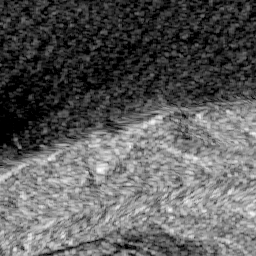
\includegraphics[width=\textwidth]{./images/sen12/ROIs1158_spring_s1_0_p19.png}
        \caption{SAR (Sentinel-1, VV)}
        \label{subfig:sen12_sar}
    \end{subfigure}
    \hspace{0.5cm}
    \begin{subfigure}[t]{0.4\textwidth}
        \centering
        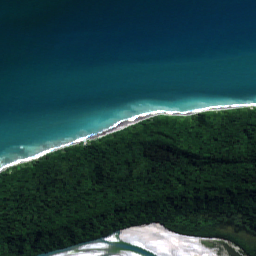
\includegraphics[width=\textwidth]{./images/sen12/ROIs1158_spring_s2_0_p19.png}
        \caption{Optical (Sentinel-2, RGB)}
        \label{subfig:sen12_opt}
    \end{subfigure}
    \vspace{0.5em}
    \begin{subfigure}[t]{0.4\textwidth}
        \centering
        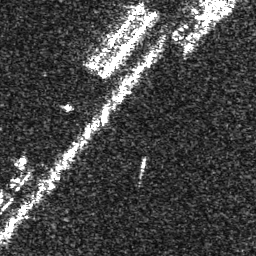
\includegraphics[width=\textwidth]{./images/qxs_sar2opt/1586_sar.png}
        \caption{SAR (Gaofen-3, VV)}
        \label{subfig:qxs_sar}
    \end{subfigure}
    \hspace{0.5cm}
    \begin{subfigure}[t]{0.4\textwidth}
        \centering
        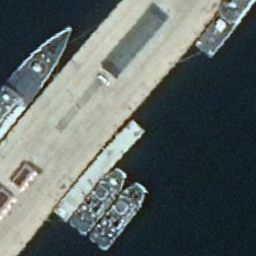
\includegraphics[width=\textwidth]{./images/qxs_sar2opt/1586_opt.png}
        \caption{Optical (Google Earth, RGB)}
        \label{subfig:qxs_opt}
    \end{subfigure}

    \caption{Примеры изображений из датасетов SEN1-2 (верхний ряд, разрешение 10~м) и QXS-SAROPT (нижний ряд, разрешение 1~м). Левый столбец: радиолокационные снимки (SAR); правый столбец: оптические снимки (Optical).}
    \label{fig:datasets_comparison_grid}
\end{figure}

\section{Выводы по третьей главе}
В главе представлено подробное описание экспериментальной базы исследования: датасетов SEN1-2 и QXS-SAROPT, включая их структуру, формат данных и обоснование выбора подмножеств.
Сформулирована формальная постановка задачи трансфера SAR $\rightarrow$ Optical.
Приведены определения и формулы для расчёта метрик, используемых для количественной оценки качества синтезируемых изображений и стандартные функции потерь, составляющие фундамент для построения конкретных архитектур.
Изложенные в настоящей главе материалы и методы служат основой для анализа общих подходов к решению задачи трансфера, проводимого в следующей главе.

\newpage